% !TEX encoding = UTF-8 Unicode
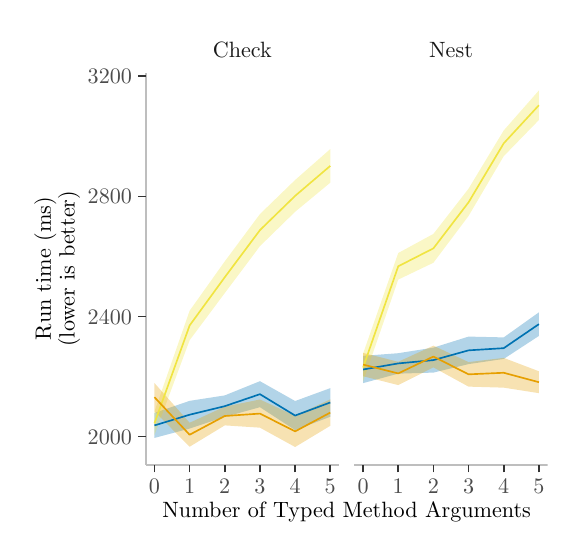
\begin{tikzpicture}[x=1pt,y=1pt]
\definecolor{fillColor}{RGB}{255,255,255}
\path[use as bounding box,fill=fillColor,fill opacity=0.00] (0,0) rectangle (187.90,180.67);
\begin{scope}
\path[clip] ( 42.64, 22.70) rectangle (112.52,164.42);
\definecolor{fillColor}{RGB}{0,114,178}

\path[fill=fillColor,fill opacity=0.30] ( 45.81, 41.46) --
	( 58.52, 45.82) --
	( 71.22, 47.79) --
	( 83.93, 52.93) --
	( 96.64, 45.76) --
	(109.34, 50.41) --
	(109.34, 40.07) --
	( 96.64, 35.25) --
	( 83.93, 43.53) --
	( 71.22, 40.01) --
	( 58.52, 35.81) --
	( 45.81, 32.42) --
	cycle;
\definecolor{fillColor}{RGB}{240,228,66}

\path[fill=fillColor,fill opacity=0.30] ( 45.81, 41.93) --
	( 58.52, 78.39) --
	( 71.22, 96.22) --
	( 83.93,113.31) --
	( 96.64,125.63) --
	(109.34,136.80) --
	(109.34,124.65) --
	( 96.64,114.14) --
	( 83.93,101.72) --
	( 71.22, 84.77) --
	( 58.52, 67.72) --
	( 45.81, 33.48) --
	cycle;
\definecolor{fillColor}{RGB}{230,159,0}

\path[fill=fillColor,fill opacity=0.30] ( 45.81, 52.25) --
	( 58.52, 37.91) --
	( 71.22, 43.74) --
	( 83.93, 46.31) --
	( 96.64, 40.44) --
	(109.34, 46.37) --
	(109.34, 36.80) --
	( 96.64, 29.14) --
	( 83.93, 36.13) --
	( 71.22, 36.96) --
	( 58.52, 29.24) --
	( 45.81, 42.03) --
	cycle;
\definecolor{drawColor}{RGB}{0,114,178}

\path[draw=drawColor,line width= 0.6pt,line join=round] ( 45.81, 36.94) --
	( 58.52, 40.81) --
	( 71.22, 43.90) --
	( 83.93, 48.23) --
	( 96.64, 40.51) --
	(109.34, 45.24);
\definecolor{drawColor}{RGB}{240,228,66}

\path[draw=drawColor,line width= 0.6pt,line join=round] ( 45.81, 37.70) --
	( 58.52, 73.06) --
	( 71.22, 90.49) --
	( 83.93,107.51) --
	( 96.64,119.88) --
	(109.34,130.73);
\definecolor{drawColor}{RGB}{230,159,0}

\path[draw=drawColor,line width= 0.6pt,line join=round] ( 45.81, 47.14) --
	( 58.52, 33.57) --
	( 71.22, 40.35) --
	( 83.93, 41.22) --
	( 96.64, 34.79) --
	(109.34, 41.58);
\end{scope}
\begin{scope}
\path[clip] (118.02, 22.70) rectangle (187.90,164.42);
\definecolor{fillColor}{RGB}{0,114,178}

\path[fill=fillColor,fill opacity=0.30] (121.20, 62.07) --
	(133.90, 63.04) --
	(146.61, 65.05) --
	(159.31, 69.04) --
	(172.02, 68.75) --
	(184.73, 77.81) --
	(184.73, 69.28) --
	(172.02, 60.97) --
	(159.31, 59.10) --
	(146.61, 56.03) --
	(133.90, 55.65) --
	(121.20, 52.23) --
	cycle;
\definecolor{fillColor}{RGB}{240,228,66}

\path[fill=fillColor,fill opacity=0.30] (121.20, 62.91) --
	(133.90, 99.24) --
	(146.61,106.15) --
	(159.31,122.49) --
	(172.02,143.54) --
	(184.73,157.98) --
	(184.73,147.30) --
	(172.02,134.23) --
	(159.31,112.63) --
	(146.61, 95.72) --
	(133.90, 89.64) --
	(121.20, 52.80) --
	cycle;
\definecolor{fillColor}{RGB}{230,159,0}

\path[fill=fillColor,fill opacity=0.30] (121.20, 63.15) --
	(133.90, 59.94) --
	(146.61, 65.77) --
	(159.31, 59.83) --
	(172.02, 61.35) --
	(184.73, 56.51) --
	(184.73, 48.60) --
	(172.02, 50.59) --
	(159.31, 50.96) --
	(146.61, 57.91) --
	(133.90, 51.52) --
	(121.20, 54.72) --
	cycle;
\definecolor{drawColor}{RGB}{0,114,178}

\path[draw=drawColor,line width= 0.6pt,line join=round] (121.20, 57.15) --
	(133.90, 59.35) --
	(146.61, 60.54) --
	(159.31, 64.07) --
	(172.02, 64.86) --
	(184.73, 73.54);
\definecolor{drawColor}{RGB}{240,228,66}

\path[draw=drawColor,line width= 0.6pt,line join=round] (121.20, 57.86) --
	(133.90, 94.44) --
	(146.61,100.93) --
	(159.31,117.56) --
	(172.02,138.88) --
	(184.73,152.64);
\definecolor{drawColor}{RGB}{230,159,0}

\path[draw=drawColor,line width= 0.6pt,line join=round] (121.20, 58.93) --
	(133.90, 55.73) --
	(146.61, 61.84) --
	(159.31, 55.40) --
	(172.02, 55.97) --
	(184.73, 52.56);
\end{scope}
\begin{scope}
\path[clip] ( 42.64,164.42) rectangle (112.52,180.67);
\definecolor{drawColor}{gray}{0.10}

\node[text=drawColor,anchor=base,inner sep=0pt, outer sep=0pt, scale=  0.80] at ( 77.58,169.79) {Check};
\end{scope}
\begin{scope}
\path[clip] (118.02,164.42) rectangle (187.90,180.67);
\definecolor{drawColor}{gray}{0.10}

\node[text=drawColor,anchor=base,inner sep=0pt, outer sep=0pt, scale=  0.80] at (152.96,169.79) {Nest};
\end{scope}
\begin{scope}
\path[clip] (  0.00,  0.00) rectangle (187.90,180.67);
\definecolor{drawColor}{RGB}{190,190,190}

\path[draw=drawColor,line width= 0.6pt,line join=round] ( 42.64, 22.70) --
	(112.52, 22.70);
\end{scope}
\begin{scope}
\path[clip] (  0.00,  0.00) rectangle (187.90,180.67);
\definecolor{drawColor}{gray}{0.20}

\path[draw=drawColor,line width= 0.6pt,line join=round] ( 45.81, 19.95) --
	( 45.81, 22.70);

\path[draw=drawColor,line width= 0.6pt,line join=round] ( 58.52, 19.95) --
	( 58.52, 22.70);

\path[draw=drawColor,line width= 0.6pt,line join=round] ( 71.22, 19.95) --
	( 71.22, 22.70);

\path[draw=drawColor,line width= 0.6pt,line join=round] ( 83.93, 19.95) --
	( 83.93, 22.70);

\path[draw=drawColor,line width= 0.6pt,line join=round] ( 96.64, 19.95) --
	( 96.64, 22.70);

\path[draw=drawColor,line width= 0.6pt,line join=round] (109.34, 19.95) --
	(109.34, 22.70);
\end{scope}
\begin{scope}
\path[clip] (  0.00,  0.00) rectangle (187.90,180.67);
\definecolor{drawColor}{gray}{0.30}

\node[text=drawColor,anchor=base,inner sep=0pt, outer sep=0pt, scale=  0.80] at ( 45.81, 12.24) {0};

\node[text=drawColor,anchor=base,inner sep=0pt, outer sep=0pt, scale=  0.80] at ( 58.52, 12.24) {1};

\node[text=drawColor,anchor=base,inner sep=0pt, outer sep=0pt, scale=  0.80] at ( 71.22, 12.24) {2};

\node[text=drawColor,anchor=base,inner sep=0pt, outer sep=0pt, scale=  0.80] at ( 83.93, 12.24) {3};

\node[text=drawColor,anchor=base,inner sep=0pt, outer sep=0pt, scale=  0.80] at ( 96.64, 12.24) {4};

\node[text=drawColor,anchor=base,inner sep=0pt, outer sep=0pt, scale=  0.80] at (109.34, 12.24) {5};
\end{scope}
\begin{scope}
\path[clip] (  0.00,  0.00) rectangle (187.90,180.67);
\definecolor{drawColor}{RGB}{190,190,190}

\path[draw=drawColor,line width= 0.6pt,line join=round] (118.02, 22.70) --
	(187.90, 22.70);
\end{scope}
\begin{scope}
\path[clip] (  0.00,  0.00) rectangle (187.90,180.67);
\definecolor{drawColor}{gray}{0.20}

\path[draw=drawColor,line width= 0.6pt,line join=round] (121.20, 19.95) --
	(121.20, 22.70);

\path[draw=drawColor,line width= 0.6pt,line join=round] (133.90, 19.95) --
	(133.90, 22.70);

\path[draw=drawColor,line width= 0.6pt,line join=round] (146.61, 19.95) --
	(146.61, 22.70);

\path[draw=drawColor,line width= 0.6pt,line join=round] (159.31, 19.95) --
	(159.31, 22.70);

\path[draw=drawColor,line width= 0.6pt,line join=round] (172.02, 19.95) --
	(172.02, 22.70);

\path[draw=drawColor,line width= 0.6pt,line join=round] (184.73, 19.95) --
	(184.73, 22.70);
\end{scope}
\begin{scope}
\path[clip] (  0.00,  0.00) rectangle (187.90,180.67);
\definecolor{drawColor}{gray}{0.30}

\node[text=drawColor,anchor=base,inner sep=0pt, outer sep=0pt, scale=  0.80] at (121.20, 12.24) {0};

\node[text=drawColor,anchor=base,inner sep=0pt, outer sep=0pt, scale=  0.80] at (133.90, 12.24) {1};

\node[text=drawColor,anchor=base,inner sep=0pt, outer sep=0pt, scale=  0.80] at (146.61, 12.24) {2};

\node[text=drawColor,anchor=base,inner sep=0pt, outer sep=0pt, scale=  0.80] at (159.31, 12.24) {3};

\node[text=drawColor,anchor=base,inner sep=0pt, outer sep=0pt, scale=  0.80] at (172.02, 12.24) {4};

\node[text=drawColor,anchor=base,inner sep=0pt, outer sep=0pt, scale=  0.80] at (184.73, 12.24) {5};
\end{scope}
\begin{scope}
\path[clip] (  0.00,  0.00) rectangle (187.90,180.67);
\definecolor{drawColor}{RGB}{190,190,190}

\path[draw=drawColor,line width= 0.6pt,line join=round] ( 42.64, 22.70) --
	( 42.64,164.42);
\end{scope}
\begin{scope}
\path[clip] (  0.00,  0.00) rectangle (187.90,180.67);
\definecolor{drawColor}{gray}{0.30}

\node[text=drawColor,anchor=base east,inner sep=0pt, outer sep=0pt, scale=  0.80] at ( 37.69, 30.12) {2000};

\node[text=drawColor,anchor=base east,inner sep=0pt, outer sep=0pt, scale=  0.80] at ( 37.69, 73.54) {2400};

\node[text=drawColor,anchor=base east,inner sep=0pt, outer sep=0pt, scale=  0.80] at ( 37.69,116.96) {2800};

\node[text=drawColor,anchor=base east,inner sep=0pt, outer sep=0pt, scale=  0.80] at ( 37.69,160.37) {3200};
\end{scope}
\begin{scope}
\path[clip] (  0.00,  0.00) rectangle (187.90,180.67);
\definecolor{drawColor}{gray}{0.20}

\path[draw=drawColor,line width= 0.6pt,line join=round] ( 39.89, 32.88) --
	( 42.64, 32.88);

\path[draw=drawColor,line width= 0.6pt,line join=round] ( 39.89, 76.29) --
	( 42.64, 76.29);

\path[draw=drawColor,line width= 0.6pt,line join=round] ( 39.89,119.71) --
	( 42.64,119.71);

\path[draw=drawColor,line width= 0.6pt,line join=round] ( 39.89,163.13) --
	( 42.64,163.13);
\end{scope}
\begin{scope}
\path[clip] (  0.00,  0.00) rectangle (187.90,180.67);
\definecolor{drawColor}{RGB}{0,0,0}

\node[text=drawColor,anchor=base,inner sep=0pt, outer sep=0pt, scale=  0.80] at (115.27,  3.82) {Number of Typed Method Arguments};
\end{scope}
\begin{scope}
\path[clip] (  0.00,  0.00) rectangle (187.90,180.67);
\definecolor{drawColor}{RGB}{0,0,0}

\node[text=drawColor,rotate= 90.00,anchor=base,inner sep=0pt, outer sep=0pt, scale=  0.80] at (  8.36, 93.56) {Run time (ms)};

\node[text=drawColor,rotate= 90.00,anchor=base,inner sep=0pt, outer sep=0pt, scale=  0.80] at ( 17.00, 93.56) {(lower is better)};
\end{scope}
\end{tikzpicture}
